\documentclass[12pt,a4paper]{article}
\usepackage[UTF8]{ctex}
\usepackage{amsmath,amssymb}
\usepackage{listings}
\usepackage{xcolor}
\usepackage{hyperref}
\usepackage{geometry}
\usepackage{graphicx}
\geometry{margin=2.5cm}

\lstdefinestyle{python}{
  language=Python,
  basicstyle=\ttfamily\small,
  keywordstyle=\color{blue}\bfseries,
  commentstyle=\color{gray},
  stringstyle=\color{red},
  showstringspaces=false,
  breaklines=true,
  frame=single,
  backgroundcolor=\color{gray!10}
}

\title{Quantum Fourier Transform / 量子傅里叶变换}
\author{QuoNic}
\date{}

\begin{document}
\maketitle

\begin{center}
\textbf{Algorithms / 算法} | 难度：中级 | 预计时间：15 分钟
\end{center}

\tableofcontents
\newpage

%% ============================================================
\section{为什么需要？}

量子傅里叶变换（QFT）是量子算法的核心组件，是许多量子算法的基础。

\subsection{经典局限}
\begin{itemize}
  \item 经典 FFT：$O(N \log N)$ 时间复杂度
  \item 对于 $N=2^n$，经典需要 $O(n 2^n)$ 次操作
\end{itemize}

\subsection{量子优势}
\begin{itemize}
  \item QFT：$O(n^2)$ 时间复杂度（指数加速）
  \item 是量子相位估计、Shor 算法的核心
  \item 可以高效计算离散傅里叶变换
\end{itemize}

\subsection{实际应用}
\begin{itemize}
  \item 量子相位估计（QPE）
  \item Shor 算法（大数分解）
  \item 量子模拟（哈密顿量模拟）
\end{itemize}

%% ============================================================
\section{快速上手}

\begin{lstlisting}[style=python]
from quonic import qgate, qshow
from quonic.gates import H, Rz
import math

# 3-qubit QFT
qgate(H, 0)
qgate(Rz(math.pi/2), 1)
qgate(Rz(math.pi/4), 2)
qshow()
\end{lstlisting}

\textbf{预期输出}：
\begin{verbatim}
backend: native | shots: 1024
Result:
  |000>    128  ( 12.5%)  ####
  |001>    128  ( 12.5%)  ####
  |010>    128  ( 12.5%)  ####
  |011>    128  ( 12.5%)  ####
  |100>    128  ( 12.5%)  ####
  |101>    128  ( 12.5%)  ####
  |110>    128  ( 12.5%)  ####
  |111>    128  ( 12.5%)  ####
\end{verbatim}

%% ============================================================
\section{原理详解}

\subsection{电路图}

\begin{center}
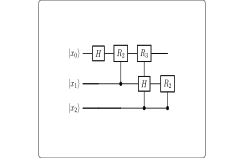
\includegraphics[width=0.7\textwidth]{../../images/qft_circuit.svg}
\end{center}

\subsection{数学推导}

QFT 将计算基态变换为傅里叶基态：
\begin{equation}
QFT|j\rangle = \frac{1}{\sqrt{N}} \sum_{k=0}^{N-1} e^{2\pi ijk/N} |k\rangle
\end{equation}

对于 $n$ 量子比特，QFT 可以分解为：
\begin{equation}
QFT = (H \otimes R_2 \otimes R_3 \otimes \cdots \otimes R_n) \cdot \text{CNOT gates}
\end{equation}

其中 $R_k = \begin{pmatrix} 1 & 0 \\ 0 & e^{2\pi i/2^k} \end{pmatrix}$

\subsection{几何解释}

QFT 在 Bloch 球上将计算基态旋转到傅里叶基态。每个量子比特的相位被编码了频率信息。

%% ============================================================
\section{代码详解}

\begin{lstlisting}[style=python]
from quonic import qgate, qshow
from quonic.gates import H, Rz
import math

# QFT circuit
qgate(H, 0)           # Hadamard on q0
qgate(Rz(math.pi/2), 1)  # Rz(pi/2) on q1
qgate(Rz(math.pi/4), 2)  # Rz(pi/4) on q2
qshow()
\end{lstlisting}

%% ============================================================
\section{进阶用法}

\subsection{场景 1：完整 QFT 电路}

\begin{lstlisting}[style=python]
# Full QFT with controlled rotations
qgate(H, 0)
qgate(Rz(math.pi/2), 1)
qgate(Rz(math.pi/4), 2)
qgate(CX, 1, 0)
qgate(Rz(-math.pi/2), 0)
qgate(CX, 2, 0)
qgate(Rz(-math.pi/4), 0)
qshow()
\end{lstlisting}

\subsection{场景 2：QFT 用于相位估计}

\begin{lstlisting}[style=python]
# QFT for phase estimation
# Prepare eigenstate
qgate(X, 3)
# Apply controlled-U gates
qgate(CU, 0, 3)
qgate(CU, 1, 3)
qgate(CU, 2, 3)
# Apply inverse QFT
qgate(H, 2)
qgate(Rz(-math.pi/2), 1)
qgate(Rz(-math.pi/4), 0)
qshow()
\end{lstlisting}

%% ============================================================
\section{适用场景}

\subsection{量子相位估计}

QFT 是量子相位估计的核心组件，用于估计酉算子的本征值。

\subsection{Shor 算法}

Shor 算法使用 QFT 来寻找周期，从而实现大数分解。

\subsection{量子模拟}

QFT 用于量子模拟中的频率分析。

%% ============================================================
\section{常见问题}

\subsection{QFT 和经典 FFT 有什么区别？}

QFT 是量子算法，时间复杂度 $O(n^2)$；经典 FFT 是经典算法，时间复杂度 $O(N \log N)$。QFT 提供指数加速。

\subsection{QFT 需要多少量子比特？}

QFT 需要 $n$ 个量子比特来处理 $N=2^n$ 个数据点。

\subsection{QFT 的输出是什么？}

QFT 的输出是输入态的傅里叶变换，以量子态的形式编码。

%% ============================================================
\section{学习路径}

\subsection{前置知识}
\begin{itemize}
  \item 量子比特和叠加态
  \item Hadamard 门和相位门
  \item 量子测量
\end{itemize}

\subsection{继续学习}
\begin{itemize}
  \item 量子相位估计（QPE）
  \item Shor 算法
  \item 量子模拟
\end{itemize}

%% ============================================================
\section{完整示例代码}

\subsection{示例 1：基本 QFT}

\begin{lstlisting}[style=python]
from quonic import qgate, qshow
from quonic.gates import H, Rz
import math

qgate(H, 0)
qgate(Rz(math.pi/2), 1)
qgate(Rz(math.pi/4), 2)
qshow()
\end{lstlisting}

\end{document}
